\section{Data Samples}\label{sec::data_sample}

This analysis is based on a data sample over \lhcb Runs  2, collected between 2015-2018. The total integrated luminosity for \lhcb during this time is approximately 6.0\invfb. Data is taken from different stripping lines for different years (Tab.\ref{tab:strippings}).\\

\begin{table}[ht]
    \centering
    \begin{tabular}{c|c|c|c}
        Year & Stripping Used & Integrated luminosity (\invfb) & Energy (TeV) \\
        \hline\hline
        2015 & \texttt{Stripping24r1} & 0.328 & 6.5\\
        2016 & \texttt{Stripping28r1} & 1.665 & 6.5\\
        2017 & \texttt{Stripping29r2} & 1.609 & 6.5\\
        2018 & \texttt{Stripping34} & X.XX & 6.5\\
    \end{tabular}
    \caption{Summary of the data used in the analysis, where \sqs represents the center of the mass-energy of the proton-proton collisions}
    \label{tab:strippings}
\end{table}

Data is taken from \texttt{B02DsstKsPiLLDsst2DGammaD2HHHBeauty2CharmLine} and \texttt{B02DsstKsPiDDDsst2DGammaD2HHHBeauty2CharmLine} line in the BHADRON stripping stream which produce two sets of candidates, one set of LL candidates and one set of DD candidates. Below, in the Tab.\ref{tab:stripp_1}-Tab.\ref{tab:stripp_10} there are listed detailes of stripping selection.

\vspace{1ex}
\begin{table}[h!]
\centering
\begin{tabular}{|c|c|} \hline
\multicolumn{2}{|c|}{\bf{KS0DDDInputsBeauty2CharmFilter}}\\ \hline
PT & $\ > 250$ MeV \\ \hline
M & $ \in (467,527)\ $MeV \\ \hline
\end{tabular}
\caption{\KS downstream stripping selection.}
\label{tab:stripp_1}
\end{table}

\vspace{1ex}
\begin{table}[h!]
\centering
\begin{tabular}{|c|c|} \hline
\multicolumn{2}{|c|}{\bf{PiInputsBeauty2CharmFilter}}\\ \hline
Track $\chi^2$ & $\ < 4$ \\ \hline
PT & $ > 100\ $MeV \\ \hline
P & $ > 1000 \ $MeV \\ \hline
Min. IP & $ > 4$ \\ \hline
TRGHP & $ < 0.4$ \\ \hline
\end{tabular}
\caption{\pion from \Ds stripping selection.}
\end{table}


\vspace{1ex}
\begin{table}[h!]
\centering
\begin{tabular}{|c|c|} \hline
\multicolumn{2}{|c|}{\bf{PiPIDTopoInputsBeauty2CharmFilter}}\\ \hline
PT & $ > 500\ $MeV \\ \hline
P & $ > 5000 \ $MeV \\ \hline
\multicolumn{2}{|c|}{\bf{PiPIDInputsBeauty2CharmFilter}}\\ \hline
PIDK & $ < 20$ \\ \hline
\end{tabular}
\caption{Additional \pion stripping selection.}
\label{tab:stripp_3}
\end{table}

\vspace{1ex}
\begin{table}[h!]
\centering
\begin{tabular}{|c|c|} \hline
\multicolumn{2}{|c|}{\bf{GammaBeauty2CharmFilter}}\\ \hline
PT & $\ > 90$ MeV \\ \hline
CL & $\ > 0.25$ \\ \hline
\end{tabular}
\caption{\g stripping selection.}
\label{tab:stripp_4}
\end{table}


\vspace{1ex}
\begin{table}[h!]
\centering
\begin{tabular}{|c|c|} \hline
\multicolumn{2}{|c|}{\bf{PiInputsBeauty2CharmFilter}}\\ \hline
$\chi^2$ śladu & $\ < 4$ \\ \hline
PT & $ > 100\ $MeV \\ \hline
P & $ > 1000 \ $MeV \\ \hline
Min. IP & $ > 4$ \\ \hline
TRGHP & $ < 0.4$ \\ \hline
\end{tabular}
\begin{tabular}{|c|c|} \hline
\multicolumn{2}{|c|}{\bf{KInputsBeauty2CharmFilter}}\\ \hline
$\chi^2$ śladu & $\ < 4$ \\ \hline
PT & $ > 100\ $MeV \\ \hline
P & $ > 1000 \ $MeV \\ \hline
Min. IP & $ > 4$ mm \\ \hline
TRGHP & $ < 0.4$ \\ \hline
\end{tabular}
\paragraph{}
\begin{tabular}{|c|c|} \hline
\multicolumn{2}{|c|}{\bf{D2HHHPIDBeauty2CharmFilter}}\\ \hline
Liczba $\pi$: PIDp $\ < 10$ & = 0 \\ \hline
Liczba $\pi$: PIDK $\ > 20$ & = 0 \\ \hline
Liczba $K$: PIDK $\ < -10$ & = 0 \\ \hline
\end{tabular}
\caption{\pion and \kaon from \Ds stripping selection.}
\label{tab:stripp_6}
\end{table}


\vspace{1ex}
\begin{table}[h!]
\centering
\begin{tabular}{|c|c|} \hline
\multicolumn{2}{|c|}{\bf{Dsst2DGammaCPVD2HHHBeauty2Charm}}\\ \hline
$|\Delta_M|$ & $\in (80,250)$ MeV \\ \hline
\end{tabular}
\caption{\Dss stripping selection.}
\label{tab:stripp_7}
\end{table}

\vspace{1ex}
\begin{table}[h!]
\centering
\begin{tabular}{|c|c|} \hline
\multicolumn{2}{|c|}{\bf{B02DsstKsPiDDDsst2DGammaD2HHHBeauty2Charm}}\\ \hline
$\chi^2$ śladu & $ < 4 \ $ \\ \hline
DIRA & $ > \ 0.999$ \\ \hline
$\tau$  & $ > \ 0.2 \ $ps \\ \hline
IP $\chi^2$ & $<25$ \\ \hline
PT & $ > 500\ $MeV \\ \hline
P & $ > 5000 \ $MeV \\ \hline
BPVVDCHI2 & $ > 1000$ \\ \hline
VFASPF(VCHI2/VDOF) & $ < 10$ \\ \hline
\end{tabular}
\caption{\Bs stripping selection.}
\label{tab:stripp_8}
\end{table}

\vspace{1ex}
\begin{table}[h!]
\centering
\begin{tabular}{|c|c|} \hline
\multicolumn{2}{|c|}{\bf{First \Bs daughter}}\\ \hline
P & $ > 10000\ $MeV \\ \hline
PT & $ > 1700 \ $MeV \\ \hline
$\chi^2$ śladu & $ < 4 \ $ \\ \hline
Min. IP & $ < 16 \ $ \\ \hline
Min. IP PV & $ > 0.1 \ $mm \\ \hline
\end{tabular}
\caption{\Bs daughter stripping selection.}
\label{tab:stripp_9}
\end{table}

\vspace{1ex}
\begin{table}[h!]
\centering
\begin{tabular}{|c|c|} \hline
\multicolumn{2}{|c|}{\bf{Second \Bs daughter}}\\ \hline
\ \ \ $\chi^2$ \ śladu \ \ \ & $ < 4 \ $ \\ \hline
PT & $ > 500 \ \ $MeV \\ \hline
P & $ > 5000 \ $MeV \\ \hline
\multicolumn{2}{|c|}{\bf{or}}\\ \hline
ID & $K_s^0 \ $ \\ \hline
PT & $ > 500 \ $MeV \\ \hline
\ \ \ \ P \ \ \ \ \ & $ > 5000 \ $MeV \\ \hline
\end{tabular}
\caption{\Bs daughter stripping selection.}
\label{tab:stripp_10}
\end{table}

The additional requirement was made in \Bs\to\Dss\Kstarm analysis. Since there is no stripping selection for the \Kstarm the preselection of \Kstar base on the cut on invariant mass of \KS\pim: $m(\KS\pim)< 1400$ MeV.  The Fig. \ref{fig:kstar_stripp} present invariant mass of \KS\pim candidates after $m(\KS\pim)< 1400$ MeV for 2015 data sample. The red colour indicates 75 MeV mass windows around the nominal mass of \Kstarm. Only events with \Kstarm mass within this mass window will be considered in the Bs\to\Dss\Kstarm analysis. 

\begin{figure}[h]
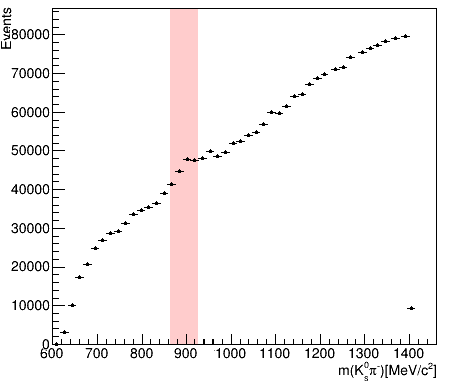
\includegraphics[width=9cm]{figs/introduction/Kstar_stripping.png}
\centering
\caption{Invariant mass of \KS\pim candidates for 2015 data sample with $m(\KS\pim)< 1400$ MeV cut. The red color indicate 75 MeV mass windows around nominal mass of \Kstarm(892)}
\label{fig:kstar_stripp}
\end{figure}



\subsection{Trigger}

All  candidates used in this analysis are required to have passed the following triggers:

\begin{itemize}
    \item \texttt{L0HadronDecision}
    \item \texttt{L0MuonDecision}
    \item \texttt{L0DiMuonDecision}
    \item \texttt{L0ElectronDecision}
    \item \texttt{L0PhotonDecision}
    \item \texttt{Hlt1TrackMVADecision}
    \item \texttt{Hlt1TwoTrackMVADecision}
    \item \texttt{Hlt2IncPhiDecision}
    \item \texttt{Hlt2Topo2BodyDecision}
    \item \texttt{Hlt2Topo3BodyDecision}
    \item \texttt{Hlt2Topo4BodyDecision}
    
\end{itemize}

\subsection{Simulated events}

Several Monte Carlo simulated samples were used in several parts of this analysis. These samples have been divided due to the method of production.  MC is generated for both the signal mode and all considered background modes. 

\subsubsection{Full simulated events}

Full simulation samples have been generated for signal and background modes. Both magnet polarities were generated, the 2016 sample was generated with Pythia8 and Sim09, the 2020 sample was generates with PythiaX and SimX. All samples were generated with all daughters in LHCb acceptance. The signal sample is produced with the \Ds decay to  \Dsp~\to\Kp\Km\pip. The specific MC data samples requested may be found in Tab.\ref{tab:MC_Full}.

\begin{table}[ht]
    \centering
    \begin{tabular}{ccccc}
        \hline
        Event type number & Year &   Decay & Options & Type\\
        \hline
        13266301 & 2016 & \Bs\to\Dss\Kstarm & \texttt{sqDalitz, DecProdCut} & DST\\
        XXXXXXX & 2020 & \Bs\to\Dss\KS\pim & \texttt{sqDalitz, DecProdCut}\\
        XXXXXXX & 2020 & \Bs\to\Dp\KS\pim & \texttt{sqDalitz, DecProdCut}\\
        13264221  & 2018 & \Bs\to\Dss\pim & \texttt{sqDalitz, DecProdCut} & DST\\
        
    \end{tabular}
    \caption{Full MC samples used  in analysis}
    \label{tab:MC_Full}
\end{table}

\subsubsection{Simplify simulated events}

The simplify simulated events have been generated using RapidSim simulation package. RapidSim allows for the fast simulation of phase space decays of beauty and charm quark hadrons, allowing quick studies of the properties of signal and background decays in physics analysis. RapidSim features generations of events using different identification hypotheses, different range of momentum, and angular acceptance of the detector.  The specific MC data samples generated using RapidSim may be found in Tab.\ref{tab:MC_Simple}.


\begin{table}[ht]
    \centering
    \begin{tabular}{ccc}
        \hline
        Sample Number &  Decay & Options\\
        \hline
        1 &  XXXXXXX  & \texttt{option}\\
    \end{tabular}
    \caption{Simplify MC samples used in analysis}
    \label{tab:MC_Simple}
\end{table}

\subsubsection{MC application in MVA}

As the simulated events pass the stripping line condition, they represent the decay signal and can be used in training of multivariate analysis method. As the number of events useful in Multivariate Analysis' method training was low (what can result in overtraining the method ..... , *multiplication?*).

\subsubsection{MC application in efficiency calculation}

Another application of simulated events is a calculation of efficiency of both selection criteria and BDT method. Efficiency is calculated for each criterion as the number of MC events that pass the requirements to the total number of simulated events.  Since the expected number of data events is low, both efficiencies should be as big as possible. Selection efficiency is used in the calculation of total efficiency, which is taken into account during relative branching fraction calculation. 